\documentclass[aspectratio=169]{beamer}
\usepackage{lmodern}
\usepackage[utf8]{inputenc}

\usepackage{enumerate}
\usepackage{multimedia}

\usetheme{polimithx}
\usepackage{natbib}
\usepackage{booktabs}
 
\title[Safe Policy Optimization]{Safe Policy Optimization\\ \vspace{0.2cm}\small{Ph.D. Course in Information Technology (Computer Science and Engineering), XXXIII cycle} \\ Second Yearly Evaluation}
\date[AAA]{\vspace{0.2cm}  30th September 2019 }
\author[M. Papini]{\textbf{Matteo Papini} \\ Supervisor: Prof. Marcello Restelli}

\begin{document}

%%%%%%%%%%%%%%%%%%%%%%%%%%%%%%%%%%%%%%%%%%%%%%%%%%%%%%%%%%%%%%%%%%%%%%%%%%%%%%%%%%%%%%%%%%%%%%%%%%%%%%%%%%%%%%%%%%%%
\begin{frame}
\titlepage
\end{frame}

\addtocounter{framenumber}{-1}

%%%%%%%%%%%%%%%%%%%%%%%%%%%%%%%%%%%%%%%%%%%%%%%%%%%%%%%%%%%%%%%%%%%%%%%%%%%%%%%%%%%%%%%%%%%%%%%%%%%%%%%%%%%%%%%%%%%%
\begin{frame}
\frametitle{Motivation}
Apply \textbf{Reinforcement Learning} to \textbf{real-world} control problems
\vfill
\centering
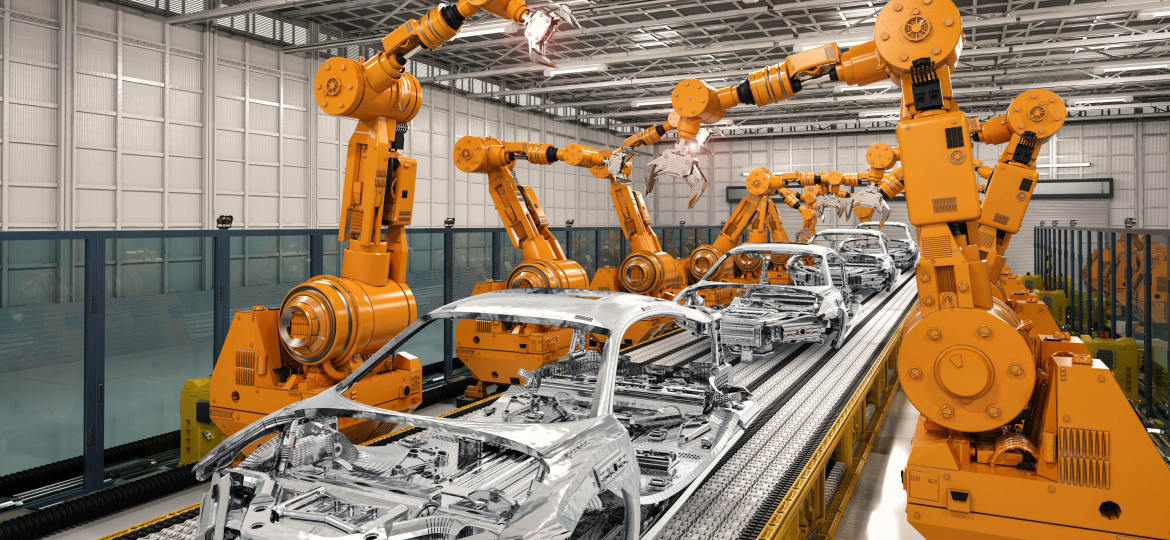
\includegraphics[width=.85\textwidth]{pics/factory.jpg}
\end{frame}

\addtocounter{framenumber}{-1}
\begin{frame}[plain]
\tableofcontents
\end{frame}

%%%%%%%%%%%%%%%%%%%%%%%%%%%%%%%%%%%%%%%%%%%%%%%%%%%%%%%%%%%%%%%%%%%%%%%%%%%%%%%%%%%%%%%%%%%%%%%%%%%%%%%%%%%%%%%%%%%
\section{Problem Definition}
\addtocounter{framenumber}{-1}
\frame[plain]{\tableofcontents[currentsection]}

\begin{frame}
\begin{overlayarea}{\textwidth}{\textheight}
\frametitle{Reinforcement Learning{\small~\citep{sutton2018reinforcement}}}
\centering
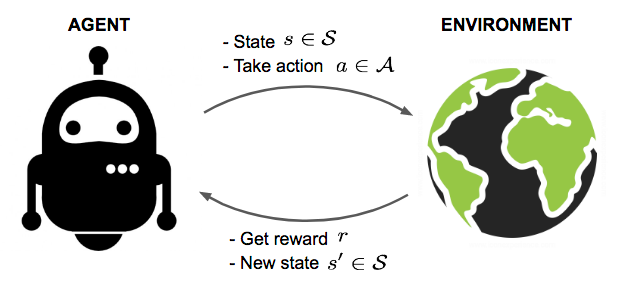
\includegraphics[width=.5\textwidth]{pics/rl2.png}\\
\vspace{.25cm}
\only<2->{
{\bf Policy $\pi$:} agent's behavior ($s\mapsto a$) \\
{\bf Performance $\rho(\pi)$:} \emph{expected} total reward \\
{\bf Goal:} find policy maximizing performance
}

\vspace{.25cm}
\only<3->{
\begin{itemize}
	\item Model-free
	\item Online
	\item Iterative
\end{itemize}
}
\end{overlayarea}
\end{frame}

\begin{frame}
\frametitle{Safety in Reinforcement Learning}
\begin{itemize}
	\setlength{\itemsep}{20pt}
	\item<1-> Many notions of safety ~\citep{amodei2016concrete,garcia2015comprehensive}
	\item<2-> Assume performance $\rho$ already encodes \emph{safety constraints}
	\item<3-> The optimal policy will be safe
	\item<4-> \textbf{The learning process itself may not be!}
\end{itemize}
\end{frame}

\begin{frame}
\frametitle{Continuous Reinforcement Learning}
\vspace{.25cm}
\begin{overlayarea}{\textwidth}{\textheight}
Interesting real-world control problems are \textbf{continuous}
\begin{center}
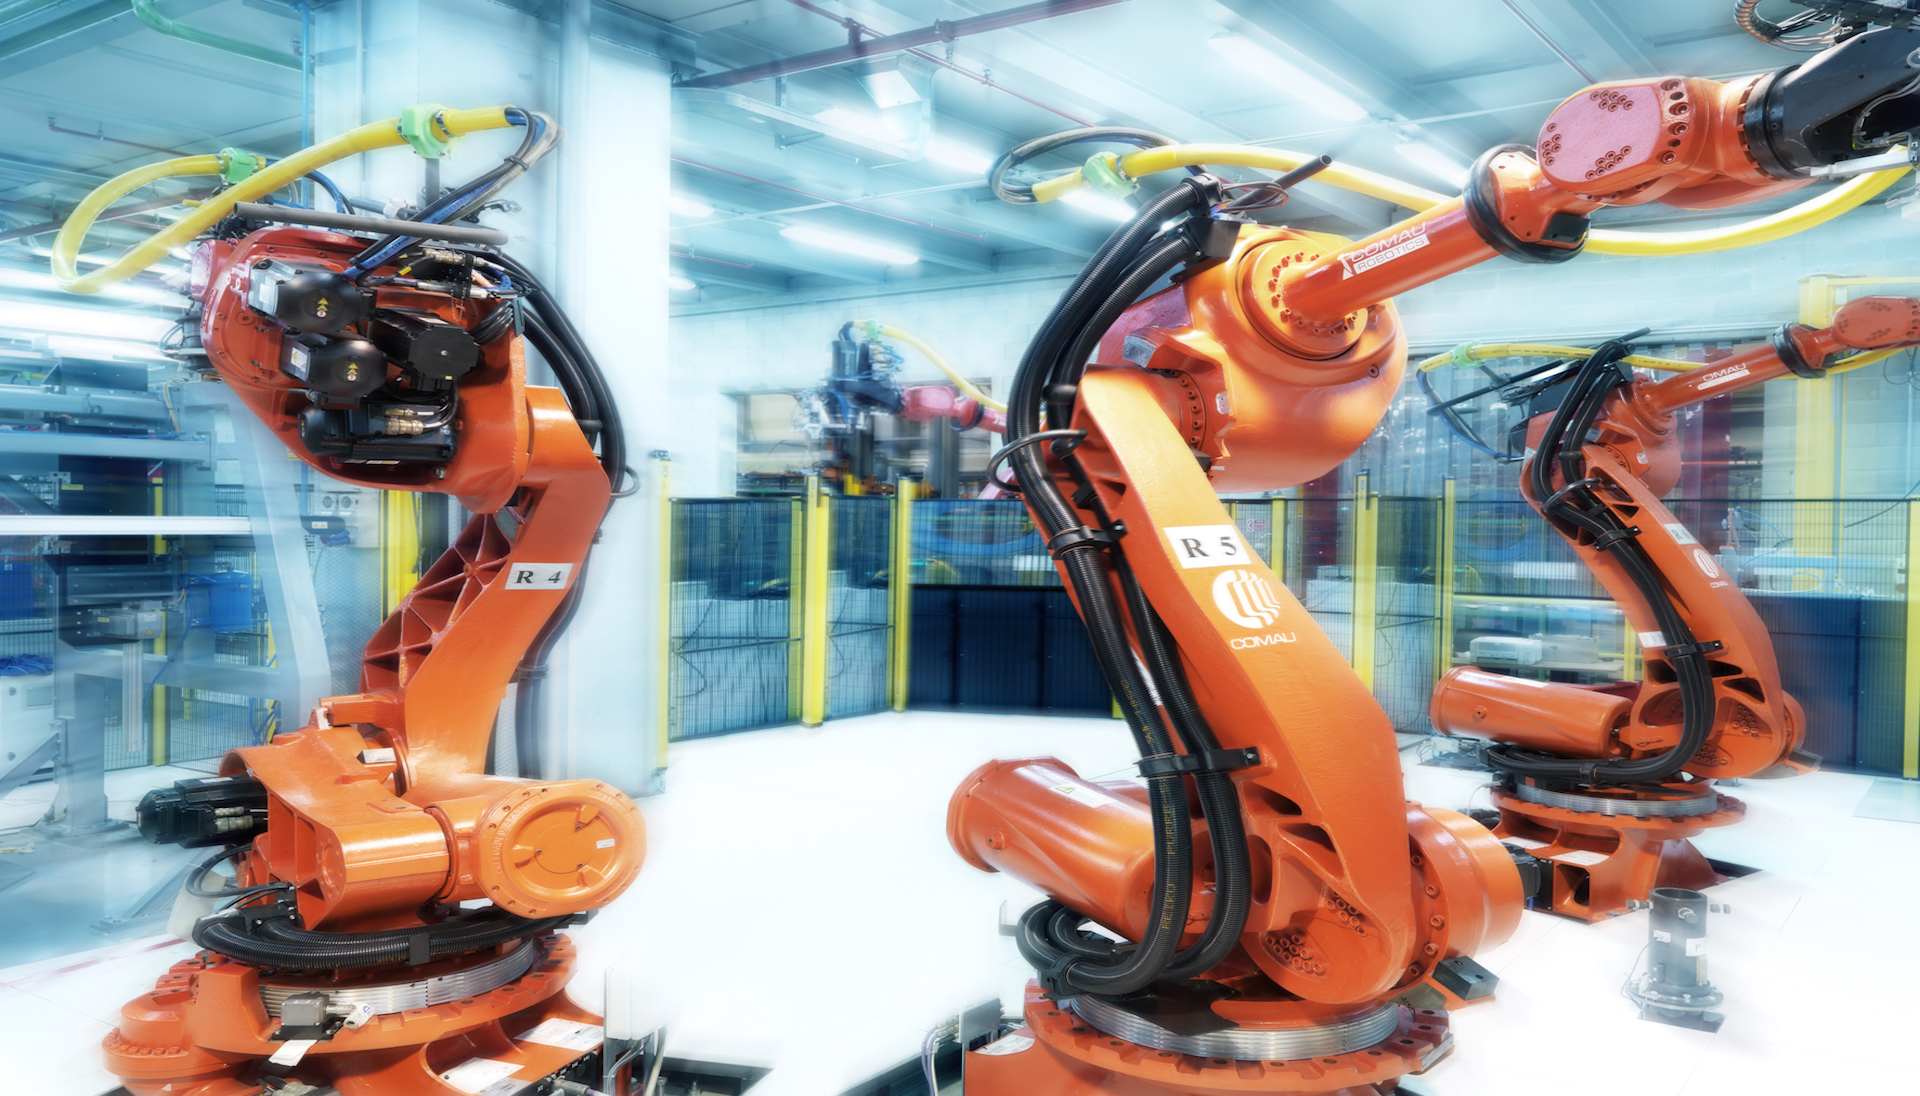
\includegraphics[width=.45\textwidth]{pics/robots.jpg}
\end{center}

\only<2->{
\textbf{Policy Optimization~\citep{deisenroth2013survey}:}
\begin{itemize}
	\item Scales well with state-action dimensionality
	\item Convergence guarantees~\citep{sutton1999policy}
	\item Robustness to noise
\end{itemize}
}
\end{overlayarea}
\end{frame}

\begin{frame}
\begin{overlayarea}{\textwidth}{\textheight}
\frametitle{Policy Optimization}
\begin{itemize}
	\item<1-> Fix a class of controllers with tunable parameters $\boldsymbol{x}\in\mathcal{X}$
	\item<2-> Find policy parameters maximizing performance:
	\vspace{-.25cm}
	\[	\Large
		\max\limits_{\boldsymbol{x}\in\mathcal{X}} \rho(\boldsymbol{x})
	\]

	\item<3-> \textbf{Policy Gradient:} solve it with \emph{Stochastic Gradient Descent}
	\vspace{.25cm}
	\only<4->{
	\begin{columns}
		\begin{column}{.5\textwidth}
			\centering
			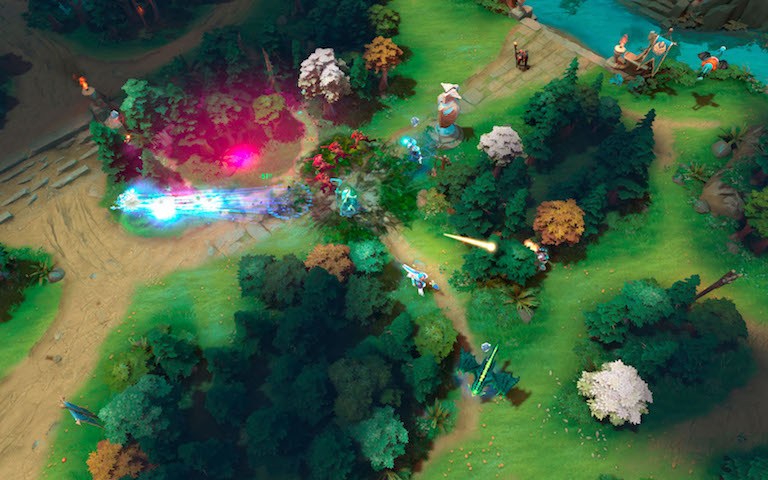
\includegraphics[width=.8\textwidth]{pics/dota.jpg}
			\\
			\emph{\cite{OpenAI_dota}}
		\end{column}
		\begin{column}{.5\textwidth}
			\centering
			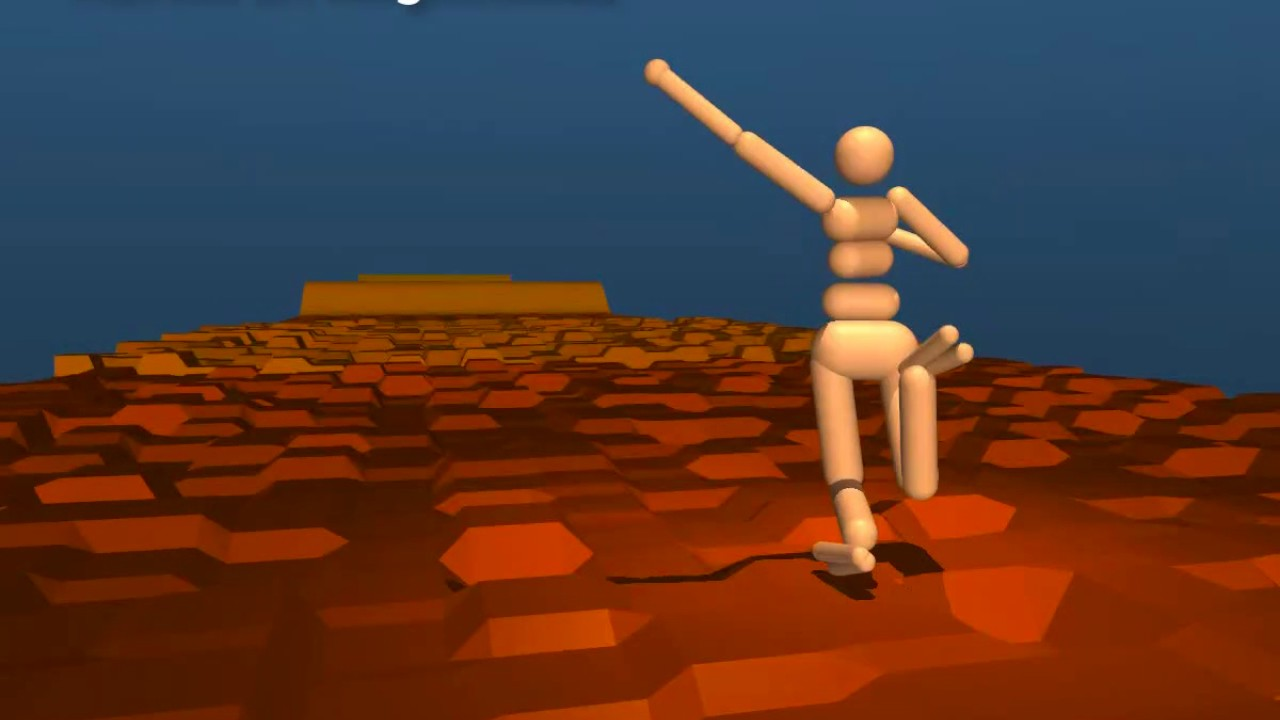
\includegraphics[width=.9\textwidth]{pics/parkour.jpg}
			\\ 
			\emph{\cite{heess2017emergence}}
		\end{column}
	\end{columns}
}
\end{itemize}
\end{overlayarea}
\end{frame}

\begin{frame}
\begin{overlayarea}{\textwidth}{\textheight}
\frametitle{Real-World Requirements}
\begin{columns}
	\begin{column}{.5\textwidth}
		{\bf ML Engineer:} "I will improve your controller with RL!"
	\end{column}
	\begin{column}{.5\textwidth}
	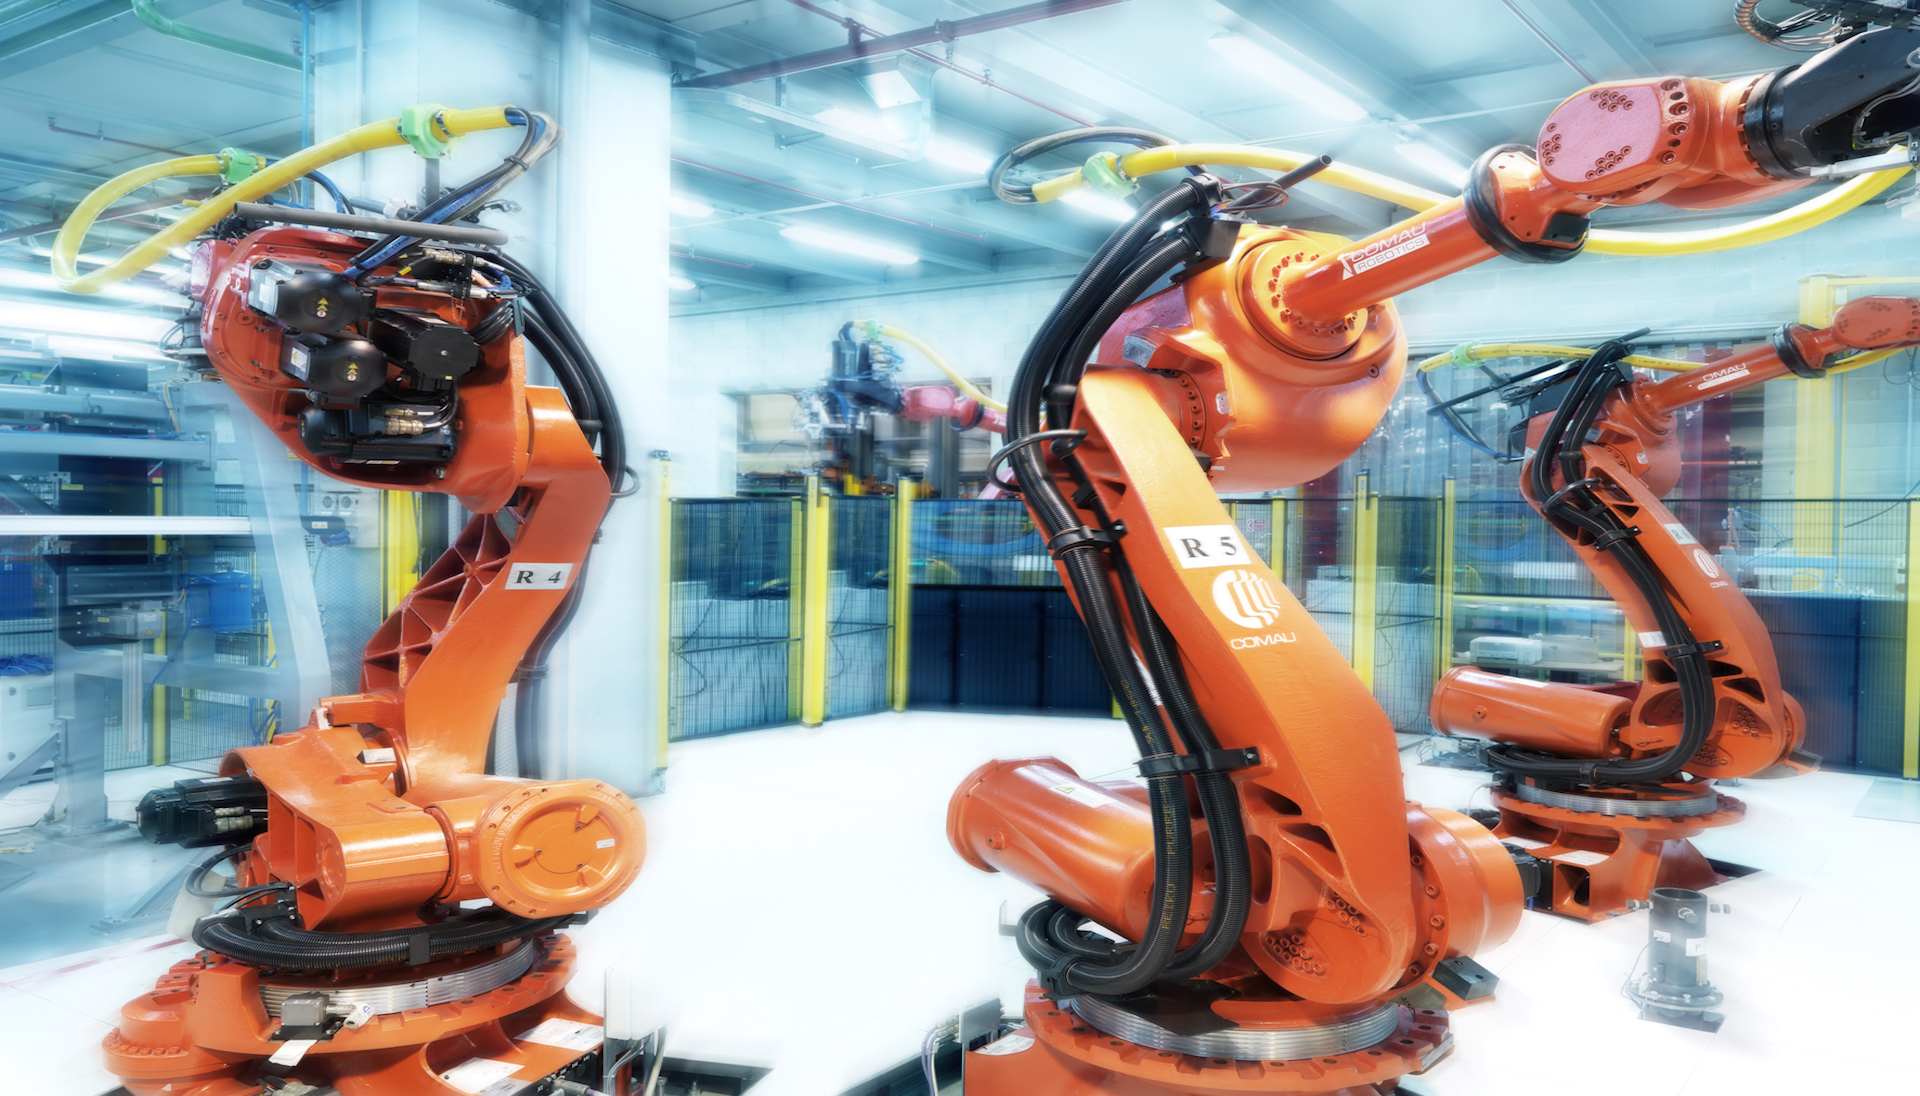
\includegraphics[width=.75\textwidth]{pics/robots.jpg}
	\end{column}
\end{columns}

%\vspace{.5cm}
\only<2->{
{\bf Boss:}\\
\begin{itemize}
	\setlength{\itemsep}{10pt}
	\item<2-> "How long will it take?" \qquad\only<6->{\textcolor{red}{Unkown}}
	\item<3-> "Will it \emph{actually} improve?"\qquad\only<7->{\textcolor{red}{Eventually}}
	\item<4-> "Will it behave safely?"\qquad\only<8->{\textcolor{red}{Eventually}}
	\item<5-> "How much better will it become?"\qquad\only<9->{\textcolor{red}{Unkown}}
\end{itemize}
}
\end{overlayarea}
\end{frame}

\section{Proposed Solutions}
\addtocounter{framenumber}{-1}
\frame{\tableofcontents[currentsection]}
\subsection{Sample Complexity}

\addtocounter{framenumber}{-1}
\begin{frame}[plain]
\begin{overlayarea}{\textwidth}{\textheight}
\vspace{2cm}
\begin{center}
	\Large
	Sample Complexity \\("How long will it take?")
\end{center}

\vspace{1cm}
\only<2->{
First year:\\
\vspace{.5cm}
\small
\textbf{Matteo Papini}, Damiano Binaghi, Giuseppe Canonaco, Matteo Pirotta, Marcello Restelli:
\emph{Stochastic Variance-Reduced Policy Gradient}. \textbf{ICML 2018}: 4023-4032

\vspace{.25cm}
Alberto Maria Metelli, \textbf{Matteo Papini}, Francesco Faccio, Marcello Restelli:
\emph{Policy Optimization via Importance Sampling}. \textbf{NeurIPS 2018}: 5447-5459
}
\end{overlayarea}
\end{frame}

%%%%%%%%%%%%%%%%%%%%%%%%%%%%%%%%%%%%%%%%%%%%%%%%%%%%%%%%%%%%%%%%%%%%%%%%%%%%%%%%%%%%%%%%%%%%%%%%%%%%%%%%%%%%%%%%%%%
\subsection{Safe Policy Updates}

\addtocounter{framenumber}{-1}
\begin{frame}[plain]
\begin{center}
	\Large
	Safe Policy Updates \\("Will it actually improve?")
\end{center}
\end{frame}


\begin{frame}
\frametitle{Monotonic Performance Improvement}
\begin{overlayarea}{\textwidth}{\textheight}
\begin{itemize}
	\item A concrete problem in Reinforcement Learning
\end{itemize}
\vspace{-.25cm}
\centering
\only<1>{
	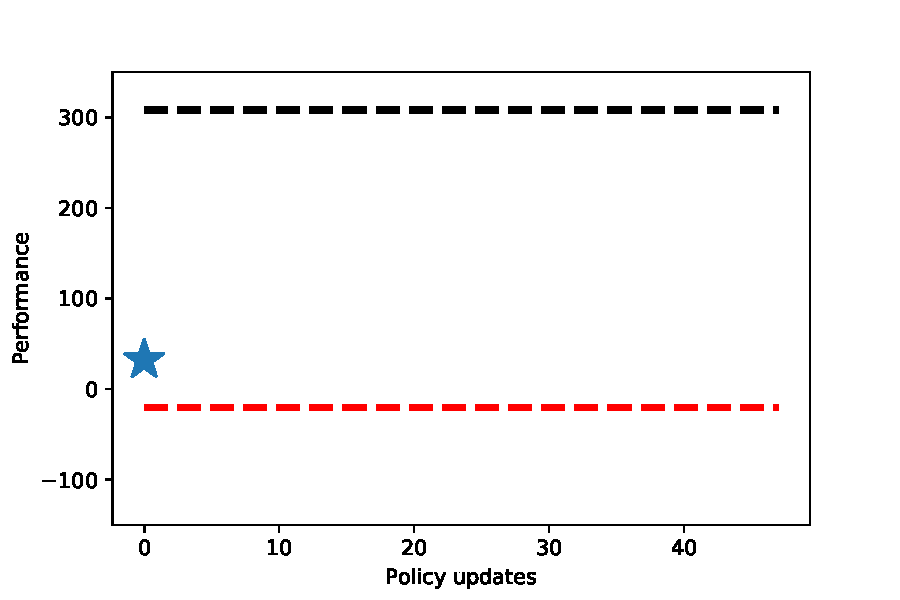
\includegraphics[width=.75\textwidth]{pics/imp1.pdf}
}
\only<2>{
	\hspace{-4pt}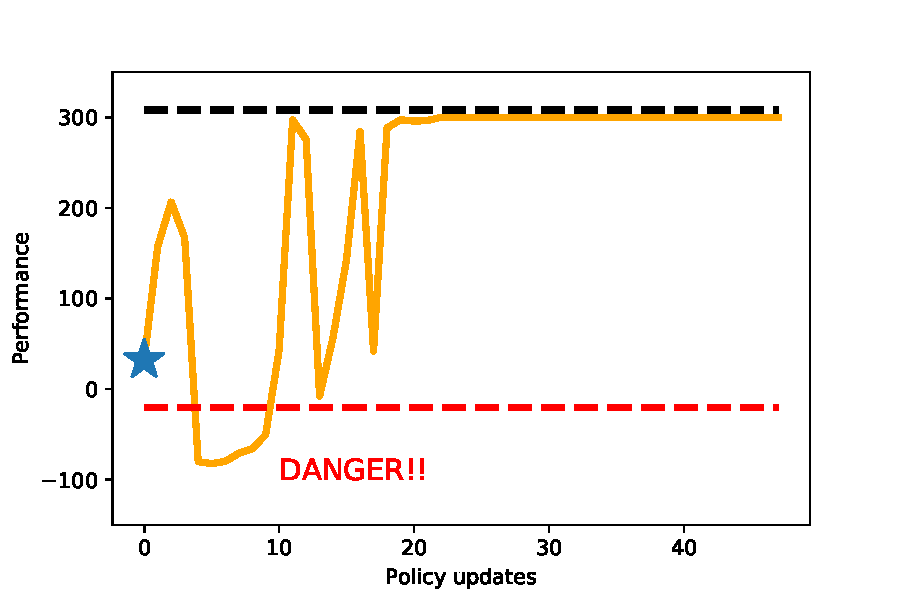
\includegraphics[width=.75\textwidth]{pics/imp2.pdf}
}
\only<3->{
	\hspace{-8pt}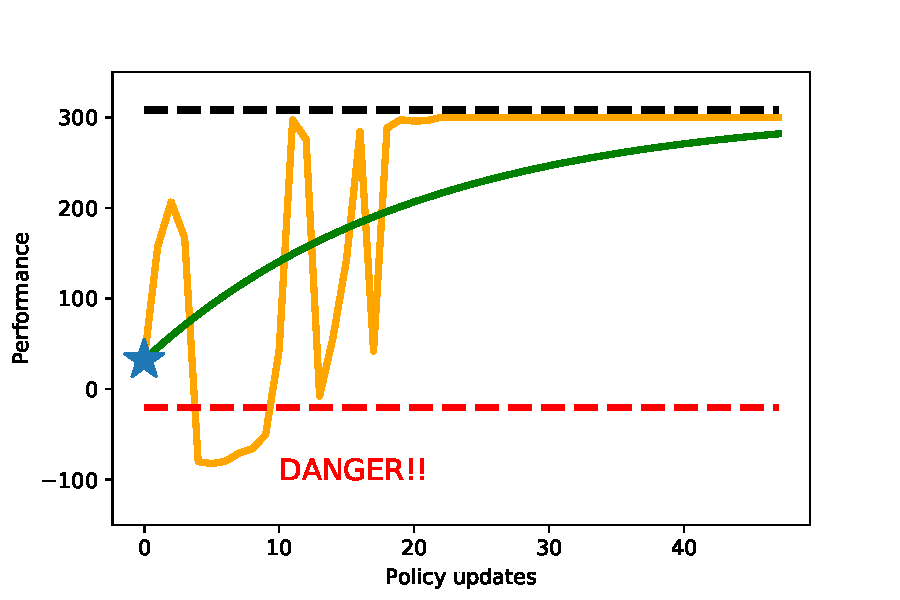
\includegraphics[width=.75\textwidth]{pics/imp3.pdf}
}
\end{overlayarea}
\end{frame}

\begin{frame}
\frametitle{Smoothing Policies and Safe Policy Gradients}
\begin{overlayarea}{\textwidth}{\textheight}
A policy gradient algorithm with \textbf{monotonic improvement} guarantees\\
\vspace{.25cm}
\only<2->{
State of the art~\citep{kakade2002approximately,pirotta2015policy,pirotta2013adaptive,schulman2015trust,papini2017adaptive}:
\begin{itemize}
	\item Restricted policy class
	\item Regularity assumptions on the environment
\end{itemize}
}
\vspace{.25cm}
\only<3->{
Our method:
\begin{itemize}
	\item General conditions on policy
	\item No assumptions on the environment
	\item Simpler formulation
	\item Smaller gap between theory and practice
\end{itemize}
}
\vspace{.5cm}
\only<3->{
\emph{Submitted to JMLR}
}
\end{overlayarea}
\end{frame}

%%%%%%%%%%%%%%%%%%%%%%%%%%%%%%%%%%%%%%%%%%%%%%%%%%%%%%%%%%%%%%%%%%%%%%%%%%%%%%%%%%%%%%%%%%%%%%%%%%%%%%%%%%%%%%%%%%%
\subsection{Safe Exploration}
\addtocounter{framenumber}{-1}
\begin{frame}[plain]
\begin{center}
	\Large
	Safe Exploration \\("Will it behave safely?")
\end{center}
\end{frame}

\begin{frame}
\frametitle{Safe Exploration}
\begin{overlayarea}{\textwidth}{\textheight}
\vspace{.5cm}	
\textbf{Exploration:} perform diverse actions to gather novel information
\begin{itemize}
	\item Necessary for improvement
	\item Tipically: perform \emph{random} actions~\citep{zafarali2019understanding}
	\item Unpredictable behavior may be \textbf{unsafe}
\end{itemize}

\vspace{1cm}
\only<2->{
Control the amount of stochasticity:
\vspace{.3cm}

\textbf{Matteo Papini}, Andrea Battistello, Marcello Restelli; \emph{“Safely Exploring Policy Gradient”}; 14th European Workshop on Reinforcement Learning (\textbf{EWRL14}), Lille, France, 2018
\vspace{.5cm}

\emph{Revised version planned for \textbf{AISTATS 2020}}
}
\end{overlayarea}
\end{frame}

%\begin{frame}
%\frametitle{Safely Exploring Policy Gradients (?)}
%\end{frame}

\begin{frame}
\frametitle{OPTIMIST}
\begin{overlayarea}{\textwidth}{\textheight}
\vspace{.5cm}	
\textbf{Direct} exploration towards interesting information

\vspace{1cm}
\only<2->{
\emph{Not} policy gradient, inspired by Multi-Armed-Bandit literature~\citep{bubeck2012regret,lattimore2018bandit}

\begin{itemize}
	\item Global convergence
	\item Still requires stochasticity
	\item Non-monotonic performance
\end{itemize}

\vspace{1cm}
\textbf{Matteo Papini}, Alberto Maria Metelli, Lorenzo Lupo, Marcello Restelli: \emph{Optimistic Policy Optimization via Multiple Importance Sampling}. \textbf{ICML 2019}: 4989-4999.
}
\end{overlayarea}
\end{frame}

\begin{frame}
\frametitle{(Truly) Deterministic Policy Gradient}
\begin{itemize}
	\setlength{\itemsep}{10pt}
	\item Is (random) exploration really necessary?
	\item Maybe not if the world is sufficiently regular
	\item \textbf{Idea}: re-use similar experience instead of sampling new one
\end{itemize}

\vfill
\emph{Planned for \textbf{ICML 2020}}
\end{frame}

%%%%%%%%%%%%%%%%%%%%%%%%%%%%%%%%%%%%%%%%%%%%%%%%%%%%%%%%%%%%%%%%%%%%%%%%%%%%%%%%%%%%%%%%%%%%%%%%%%%%%%%%%%%%%%%%%%%
\section{Future Work}
\addtocounter{framenumber}{-1}
\frame{\tableofcontents[currentsection]}
\subsection{Quality of Solutions}

\addtocounter{framenumber}{-1}
\begin{frame}[plain]
\begin{center}
	\Large
	Quality of Solutions \\("How much better will it become?")
\end{center}
\end{frame}

\begin{frame}
\frametitle{Non-Convexity}
\begin{itemize}
	\setlength{\itemsep}{5pt}
	\item<1-> The performance objective $\rho$ is \textbf{nonconvex}
	\item<2-> Policy gradient only converges to \textbf{local optima}
	\item<3> Locally optimal performance could be poor
	\item<4> Locally optimal policies may be \textbf{unsafe}
\end{itemize}
\vspace{.25cm}
\centering
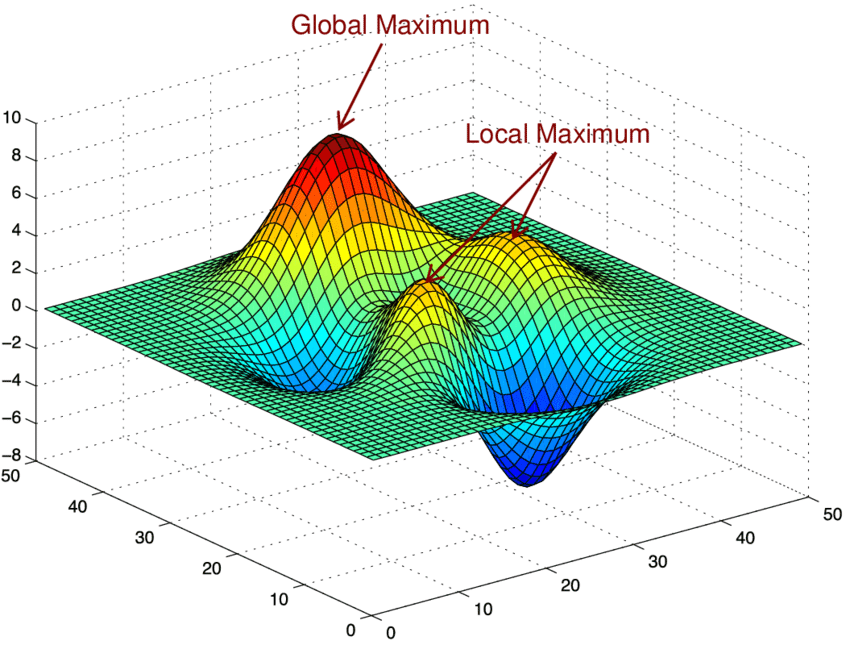
\includegraphics[width=.4\textwidth]{pics/nonconvex.png}
\end{frame}

\begin{frame}
\frametitle{Global Optimality Guarantees}
\begin{overlayarea}{\textwidth}{\textheight}
\vspace{.5cm}
\begin{itemize}
	\setlength{\itemsep}{10pt}
	\item<1-> The \emph{policy} optimization problem is \emph{special}
	\item<2-> Convergence to the \textbf{global optimum} is possible in some cases~\citep{bhandari2019global,agarwal2019optimality,shani2019adaptive}
	\item<3-> Can we exploit tools from \textbf{convex optimization} to design \emph{new} algorithms?
\end{itemize}
\vspace{.5cm}
\only<4->{
\begin{columns}
	\begin{column}{.5\textwidth}
		\centering
		Possible target: \textbf{NeurIPS 2020}
	\end{column}
	\begin{column}{.5\textwidth}
		\centering
		
\includegraphics[width=.75\textwidth]{pics/fb.jpg}
	\end{column}
\end{columns}
}
\end{overlayarea}
\end{frame}

%%%%%%%%%%%%%%%%%%%%%%%%%%%%%%%%%%%%%%%%%%%%%%%%%%%%%%%%%%%%%%%%%%%%%%%%%%%%%%%%%%%%%%%%%%%%%%%%%%%%%%%%%%%%%%%%%%%
\section{Conclusion}
\addtocounter{framenumber}{-1}
\frame{\tableofcontents[currentsection]}

\begin{frame}
\frametitle{Wrapping Up}
\begin{overlayarea}{\textwidth}{\textheight}
\begin{itemize}
	\setlength{\itemsep}{10pt}
	\item Sample Complexity~\citep{papini2018stochastic,xu2019improved,xu2019sample}
	\item Safe Policy Updates~\citep{papini2019smoothing}
	\item Safe Exploration (\cite{papini2019optimistic} + work in progress)
	\item Quality of Solutions (future work)
\end{itemize}
\vspace{1cm}
\only<2->{
We also want to:
\vspace{-1cm}
\begin{columns}
	\begin{column}{.5\textwidth}
		\begin{itemize}
			\item Find a trade-off between competing goals
			\item Apply to real problems
		\end{itemize}
	\end{column}
	\begin{column}{.5\textwidth}
		
\includegraphics[width=\textwidth]{pics/pirelli.jpg}
	\end{column}
\end{columns}
}
\end{overlayarea}
\end{frame}

\begin{frame}
\frametitle{Publications (Overview)}
\footnotesize 
\begin{table}
	\begin{tabular}{llcccc}
		& GGS & \textcolor{black!40}{2017} & 2018 & 2109 & 2020 \\
		\toprule
		\textbf{ICML} & A++ & & \citep{papini2018stochastic} & \citep{papini2019optimistic} & planed \\
		\textbf{NeurIPS} & A++ & \textcolor{black!40}{\citep{papini2017adaptive}} & \citep{metelli2018policy} & & planned \\
		\midrule
		AAAI &  A++ & & & & submitted \\
		AISTATS & A+ & & & & planned \\
		IJCNN & B & &  &\citep{beraha2019feature} & \\
		\bottomrule
	\end{tabular}
\end{table}

\end{frame}

\begin{frame}
\frametitle{Publications}
\emph{First year:}
\begin{itemize}
	\small
	\setlength{\itemsep}{10pt}
	\item  \textbf{Matteo Papini}, Damiano Binaghi, Giuseppe Canonaco, Matteo Pirotta, Marcello Restelli:
	\emph{Stochastic Variance-Reduced Policy Gradient}. \textbf{ICML 2018}: 4023-4032
	\item  Alberto Maria Metelli, \textbf{Matteo Papini}, Francesco Faccio, Marcello Restelli:
	\emph{Policy Optimization via Importance Sampling}. \textbf{NeurIPS 2018}: 5447-5459
\end{itemize}

\vfill

\emph{Second year:}
\begin{itemize}
	\small
	\setlength{\itemsep}{10pt}
	\item \textbf{Matteo Papini}, Alberto Maria Metelli, Lorenzo Lupo, Marcello Restelli:
	\emph{Optimistic Policy Optimization via Multiple Importance Sampling}. \textbf{ICML 2019}: 4989-4999
	\item Mario Beraha, Alberto Maria Metelli, \textbf{Matteo Papini}, Andrea Tirinzoni, Marcello Restelli:
	\emph{Feature Selection via Mutual Information: New Theoretical Insights}. IJCNN 2019
\end{itemize}
\end{frame}

\begin{frame}
\frametitle{Other Publications}
\emph{Before the Ph.D.:}
\begin{itemize}
	\small
	\setlength{\itemsep}{10pt}
	\item  \textbf{Matteo Papini}, Matteo Pirotta, Marcello Restelli:
	\emph{Adaptive Batch Size for Safe Policy Gradients}. \textbf{NeurIPS 2017}: 3591-3600
\end{itemize}

\vfill

\emph{Workshop papers:}
\begin{itemize}
	\small
	\item  \textbf{Matteo Papini}, Andrea Battistello, Marcello Restelli: \emph{Safely Exploring Policy Gradient}. EWRL 2018 
\end{itemize}
\end{frame}

\begin{frame}
\frametitle{Submissions}
\begin{itemize}
	\small
	\setlength{\itemsep}{10pt}
	\item  \textbf{Matteo Papini}, Matteo Pirotta, Marcello Restelli:
	\emph{Smoothing Policies and Safe Policy Gradients}. (\textbf{JMLR})
	\item  Pierluca D'Oro, Alberto Maria Metelli, Andrea Tirinzoni, \textbf{Matteo Papini}, Marcello Restelli:
	\emph{Gradient-Aware Model-based Policy Search}. (\textbf{AAAI 2020})
	\item   Lorenzo Bisi, Luca Sabbioni, Edoardo Vittori, \textbf{Matteo Papini}, Marcello Restelli: \emph{Risk-Averse Trust Region Optimization for Reward-Volatility Reduction} (\textbf{AAAI 2020})
\end{itemize}
\end{frame}

\begin{frame}
\frametitle{Courses and Schools}
\textbf{Courses (25/25 CFU):}

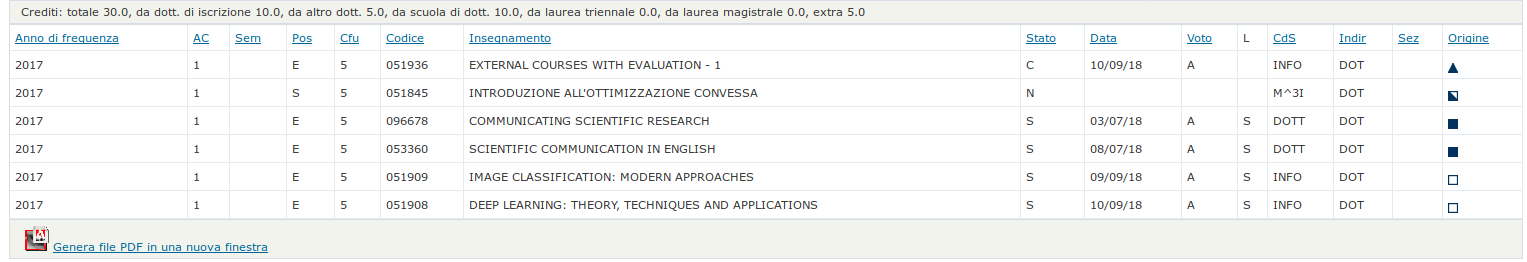
\includegraphics[width=\textwidth]{pics/corsi.png}
\vfill

\textbf{Schools:}
\begin{itemize}
	\item  Deep Learning and Reinforcement Learning Summer School (DLRLSS), Toronto, Canada, 2018
	\item  ACAI Summer School on Reinforcement Learning, Nieuwpoort, Belgium, 2017
\end{itemize}
\end{frame}

\begin{frame}
\frametitle{Teaching}
\textbf{2017/2018}
\begin{itemize}
	\setlength{\itemsep}{10pt}
	\item  Responsabile di laboratorio, Informatica B, Prof. Luca Cassano
	\item  Esercitatore, Web and Internet Economics, Prof. Nicola Gatti
\end{itemize}

\vfill
\textbf{2018/2019}
\begin{itemize}
	\setlength{\itemsep}{10pt}
	\item  Esercitatore, Informatica B, Prof. Luca Cassano
\end{itemize}

\vfill
\textbf{2019/2020}
\begin{itemize}
	\setlength{\itemsep}{10pt}
	\item  Esercitatore, Informatica B, Prof. Luca Cassano (now)
\end{itemize}

\vfill
\textbf{Teaching outside Politecnico:}
\begin{itemize}
	\setlength{\itemsep}{10pt}
	\item Teaching Assistant for the Reinforcement Learning Summer School (RLSS), Lille, France, 2019
\end{itemize}
\end{frame}

\begin{frame}
\frametitle{Other Activities}
\tiny
\textbf{Talks and posters:}
\begin{itemize}
	\item Seminar \emph{Temporal Credit Assignment in Off-Policy Reinforcement Learning}, DEIB, November 28th , 2017
	\item Poster presentation at NeurIPS 2017
	\item Oral and poster presentation at ICML 2018
	\item Poster presentation at DLRLSS 2018
	\item Poster presentation at EWRL14 (2018)
	\item Oral and poster presentation at NeurIPS 2018
	\item Oral and poster presentation at ICML 2019
	\item Invited talk at MAPLE workshop 2019
\end{itemize}

\vfill
\textbf{Editorial activities:}
\begin{itemize}
	\item Subreviewer for IJCAI 2018
	\item Reviewer for ICML 2019
	\item PC Member for UAI 2019
	\item Reviewer for NeurIPS 2019
	\item Reviewer for AAAI 2020 (now)
	\item Reviewer for AISTATS 2020 (planned)
\end{itemize}

\vfill
\textbf{Co-supervised master students:} G. Canonaco, D. Binaghi, A. Battistello, F. Faccio, A. Mongelluzzo, L. Lupo, G. Pelosi, P. Melzi (now)
\end{frame}



\begin{frame}[plain]
\centering
{\color{poliblue3} \bf
\vspace{1cm}
{\huge Thank you for your attention!} \\
\vspace{2cm}
{\LARGE Questions?}
}
\end{frame}


\begin{frame}[allowframebreaks]
\frametitle{Bibliography}
\scriptsize
\bibliographystyle{plainnat}
\bibliography{slides}
\end{frame}

%%%%%%%%%%%%%%%%%%%%%%%%%%%%%%%%%%%%%%%%%%%%%%%%%%%%%%%%%%%%%%%%%%%%%%%%%%%%%%%%%%%%%%%%%%%%%%%%%%%%%%%%%%%%%%%%%%%


\end{document} 
